\documentclass[11pt]{article}

\usepackage[margin=1in]{geometry}
\usepackage{graphicx}
\usepackage{amsmath, amssymb}
\usepackage{booktabs}
\usepackage{xcolor}
\usepackage{caption}
\usepackage[hidelinks]{hyperref}

\graphicspath{{figures/}}
\captionsetup{font=small, labelfont=bf}

\title{CS 285 Homework 5: Offline RL --- Report}
\author{Xiaolei Chu (Student ID: 3038525739)}
\date{}

\begin{document}
\maketitle

All experiments use a single seed (\texttt{seed=0}) and the default hyperparameters
shipped in the starter code (\texttt{hidden\_size=256}, \texttt{num\_layers=4},
\texttt{lr=3e-4}, \texttt{discount=0.99}, \texttt{target\_update\_rate=0.005},
\texttt{batch\_size=256}; \texttt{flow\_steps=10} for FQL; \texttt{expectile=0.9}
for IQL). Each run is trained for $10^6$ gradient steps with evaluations every
$10^5$ steps over $25$ rollouts. All numbers below are the success rates produced
by the starter-code evaluation harness.

%====================================================================
\section{SAC+BC (Section~2)}
%====================================================================

The implementation lives in \texttt{src/agents/sacbc\_agent.py}.

\paragraph{Best-performing agents.} Hyperparameter $\alpha$ was swept over
$\{30, 100, 300, 1000\}$ on \texttt{cube-single} and over $\{1, 3, 10, 30\}$ on
\texttt{antsoccer-arena}. The best run for each task is summarized in
Table~\ref{tab:q1-best} and plotted in Figure~\ref{fig:q1-best}.

\begin{table}[h]
\centering
\small
\begin{tabular}{lcccc}
\toprule
Task & Best $\alpha$ & Final success @ 1M & Best success within 1M & Pass criterion \\
\midrule
\texttt{cube-single}     & 100 & \textbf{100\%} & 100\% & $> 75\%$ final \checkmark \\
\texttt{antsoccer-arena} & 10  & 12\%           & \textbf{44\%} & $> 5\%$ \checkmark \\
\bottomrule
\end{tabular}
\caption{SAC+BC best agents.}
\label{tab:q1-best}
\end{table}

\begin{figure}[h]
\centering
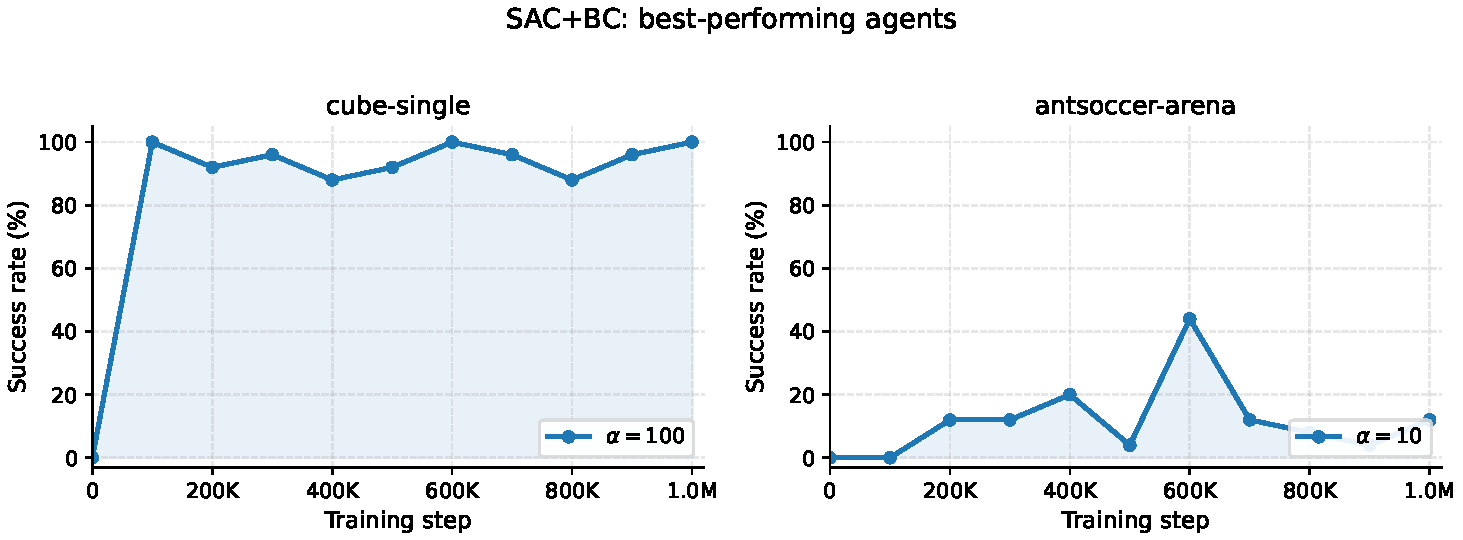
\includegraphics[width=\linewidth]{q1_best.pdf}
\caption{SAC+BC training curves of the best agents on \texttt{cube-single}
($\alpha=100$) and \texttt{antsoccer-arena} ($\alpha=10$).}
\label{fig:q1-best}
\end{figure}

\paragraph{Effect of $\alpha$ on \texttt{cube-single}.} Figure~\ref{fig:q1-sweep}
shows the four $\alpha$ values. Training is highly sensitive to $\alpha$: the
mid-range ($\alpha=100, 300$) converges fast and stays near $100\%$, the small
$\alpha=30$ (BC term too weak) is unstable around $90\%$, and the large
$\alpha=1000$ (Q maximization swamped by BC) is slower to climb and noisier.

\begin{figure}[h]
\centering
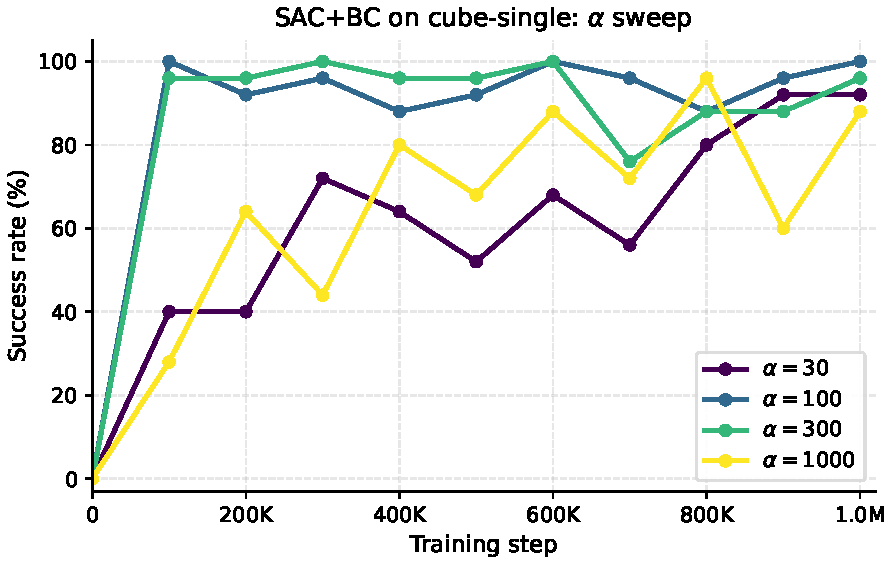
\includegraphics[width=0.7\linewidth]{q1_alpha_sweep.pdf}
\caption{SAC+BC on \texttt{cube-single} with four BC coefficients.}
\label{fig:q1-sweep}
\end{figure}

%====================================================================
\section{IQL (Section~3)}
%====================================================================

The implementation lives in \texttt{src/agents/iql\_agent.py}; the expectile
parameter is fixed at $\tau=0.9$ throughout.

\paragraph{Best-performing agents.} Inverse-temperature $\alpha$ was swept over
$\{1, 3, 10\}$ on both tasks. The best results are listed in
Table~\ref{tab:q2-best} and plotted in Figure~\ref{fig:q2-best}.

\begin{table}[h]
\centering
\small
\begin{tabular}{lcccc}
\toprule
Task & Best $\alpha$ & Final success @ 1M & Best success within 1M & Pass criterion \\
\midrule
\texttt{cube-single}     & 1  & \textbf{88\%} & 100\% & $> 60\%$ final \checkmark \\
\texttt{antsoccer-arena} & 10 & 8\%           & \textbf{36\%} & $> 5\%$ \checkmark \\
\bottomrule
\end{tabular}
\caption{IQL best agents (with $\tau=0.9$).}
\label{tab:q2-best}
\end{table}

\begin{figure}[h]
\centering
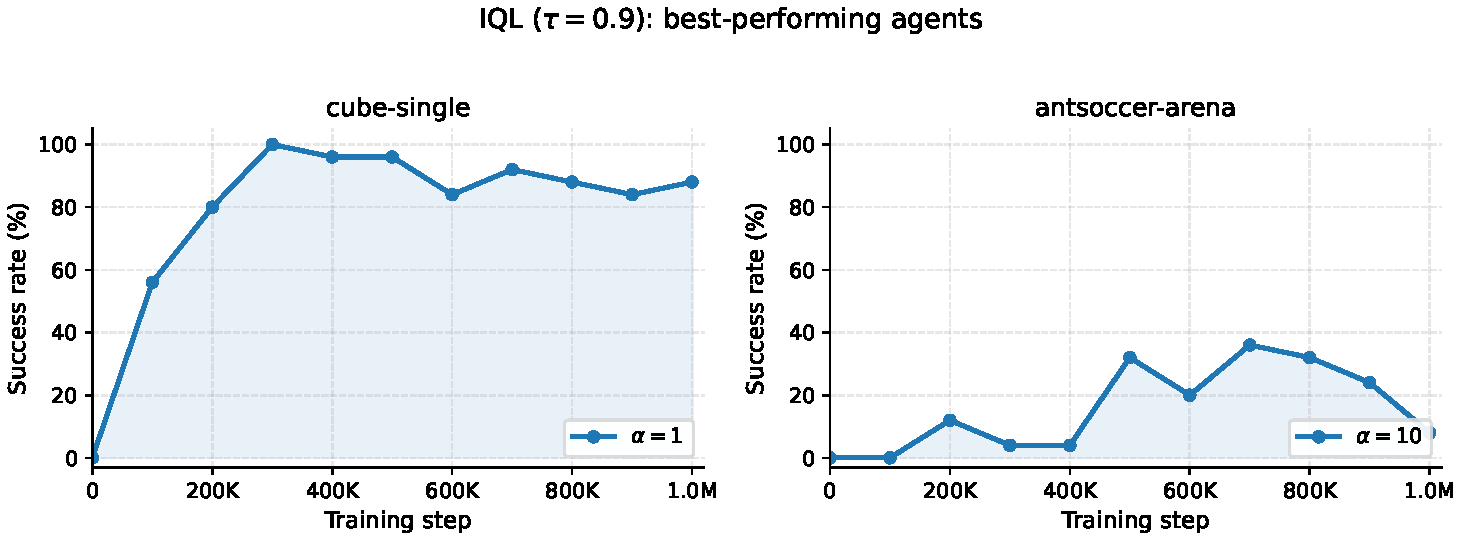
\includegraphics[width=\linewidth]{q2_best.pdf}
\caption{IQL training curves of the best agents on \texttt{cube-single}
($\alpha=1$) and \texttt{antsoccer-arena} ($\alpha=10$).}
\label{fig:q2-best}
\end{figure}

\paragraph{Effect of $\alpha$ on \texttt{cube-single}.} See
Figure~\ref{fig:q2-sweep}. All three $\alpha$ values quickly reach high success
rate; $\alpha=1$ converges to the highest plateau, while $\alpha=3, 10$ converge
to slightly lower but comparable plateaus.

\begin{figure}[h]
\centering
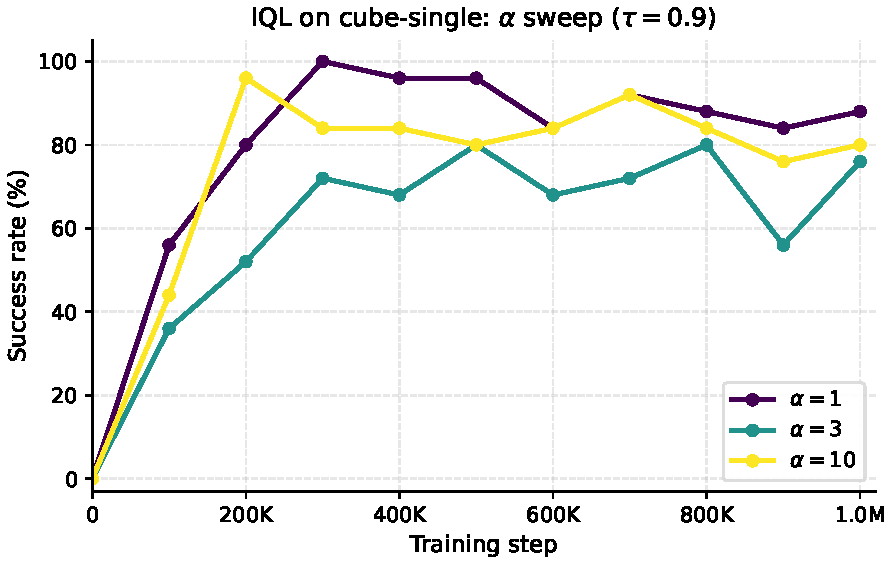
\includegraphics[width=0.7\linewidth]{q2_alpha_sweep.pdf}
\caption{IQL on \texttt{cube-single} with three inverse temperatures.}
\label{fig:q2-sweep}
\end{figure}

\paragraph{Discussion: SAC+BC vs.\ IQL.}
\textbf{(1) Best performance.} SAC+BC is slightly stronger than IQL at the
optimum on both tasks: on \texttt{cube-single} it reaches $100\%$ final success
versus IQL's $88\%$ final ($100\%$ peak); on \texttt{antsoccer-arena} the
within-1M peak is $44\%$ versus IQL's $36\%$. \textbf{(2) Sensitivity to
$\alpha$.} IQL is markedly less sensitive: all three IQL $\alpha\in\{1,3,10\}$
land within $\sim$20 percentage points of one another on \texttt{cube-single}
and all yield non-trivial success on \texttt{antsoccer-arena}, whereas SAC+BC
collapses to near-$0\%$ on \texttt{antsoccer-arena} when $\alpha$ moves to $30$
and shows much wider spread on \texttt{cube-single}. This matches the textbook
expectation that advantage-weighted regression makes IQL easier to tune.

%====================================================================
\section{FQL (Section~4)}
%====================================================================

The implementation lives in \texttt{src/agents/fql\_agent.py}.

\paragraph{Best-performing agents.} Distillation coefficient $\alpha$ was swept
over $\{30, 100, 300, 1000\}$ on \texttt{cube-single} and over $\{1, 3, 10, 30\}$
on \texttt{antsoccer-arena}. The best run for each task is given in
Table~\ref{tab:q3-best} and plotted in Figure~\ref{fig:q3-best}.

\begin{table}[h]
\centering
\small
\begin{tabular}{lcccc}
\toprule
Task & Best $\alpha$ & Final success @ 1M & Best success within 1M & Pass criterion \\
\midrule
\texttt{cube-single}     & 300 & \textbf{100\%} & 100\% & $> 80\%$ final \checkmark \\
\texttt{antsoccer-arena} & 10  & 0\%            & \textbf{52\%} & $> 30\%$ best within 1M \checkmark \\
\bottomrule
\end{tabular}
\caption{FQL best agents.}
\label{tab:q3-best}
\end{table}

\begin{figure}[h]
\centering
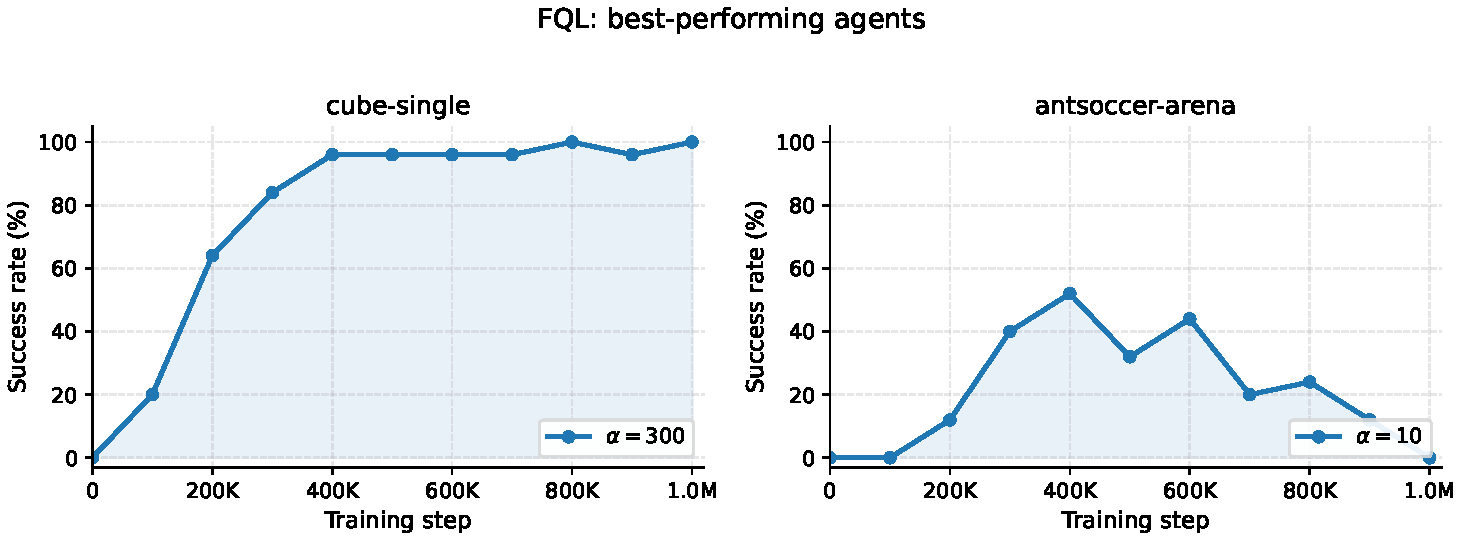
\includegraphics[width=\linewidth]{q3_best.pdf}
\caption{FQL training curves of the best agents on \texttt{cube-single}
($\alpha=300$) and \texttt{antsoccer-arena} ($\alpha=10$).}
\label{fig:q3-best}
\end{figure}

\end{document}
